\documentclass[aspectratio=169, 10pt]{beamer}

% ==============================================================================
% THEME & CLEAN MINIMALIST DESIGN SETUP (NO CRAMPED BOXES, GENEROUS BREATHING ROOM)
% ==============================================================================
\usetheme{default}
\usecolortheme{dove}

% Scientific Palette
\definecolor{NavyBlue}{RGB}{16, 44, 87}       % Primary headers
\definecolor{SlateBlue}{RGB}{35, 80, 135}     % Secondary section accents
\definecolor{EmeraldGreen}{RGB}{25, 125, 75}  % Accuracy gains / positive results
\definecolor{DarkText}{RGB}{30, 35, 45}       % Readable charcoal body text
\definecolor{SlateGray}{RGB}{115, 125, 140}   % Footline & metadata
\definecolor{LightLine}{RGB}{220, 226, 235}   % Soft divider rules

\setbeamercolor{background canvas}{bg=white}
\setbeamercolor{normal text}{fg=DarkText}
\setbeamercolor{frametitle}{fg=NavyBlue, bg=white}
\setbeamercolor{title}{fg=NavyBlue, bg=white}
\setbeamercolor{structure}{fg=SlateBlue}
\setbeamercolor{item}{fg=SlateBlue}

% Strict Uniform Typography Hierarchy Throughout Project
\setbeamerfont{title}{size=\Large, series=\bfseries}
\setbeamerfont{subtitle}{size=\small, series=\mdseries}
\setbeamerfont{frametitle}{size=\large, series=\bfseries}
\setbeamerfont{footline}{size=\scriptsize}
\setbeamerfont{footnote}{size=\scriptsize}
\setbeamerfont{caption}{size=\scriptsize}

% Remove default navigation symbols
\setbeamertemplate{navigation symbols}{}

% Clean frametitle with subtle accent divider
\setbeamertemplate{frametitle}{%
  \vspace{0.35cm}%
  {\usebeamerfont{frametitle}\insertframetitle}%
  \par%
  \vspace{0.10cm}%
  {\color{LightLine}\hrule height 0.8pt}%
  \vspace{0.12cm}%
}

% Global Footline: Strictly Uniform Size Throughout Entire Deck
\setbeamertemplate{footline}{%
  \leavevmode%
  \hbox{%
    \begin{beamercolorbox}[wd=.38\paperwidth,ht=2.5ex,dp=1.2ex,left]{footline}%
      \hspace*{3ex}\usebeamerfont{footline}\textcolor{SlateGray}{MAC-RGBD-VIO \textbar\ Target: IEEE RA-L}
    \end{beamercolorbox}%
    \begin{beamercolorbox}[wd=.34\paperwidth,ht=2.5ex,dp=1.2ex,center]{footline}%
      \usebeamerfont{footline}\textcolor{SlateGray}{Robotics Research Laboratory}
    \end{beamercolorbox}%
    \begin{beamercolorbox}[wd=.28\paperwidth,ht=2.5ex,dp=1.2ex,right]{footline}%
      \usebeamerfont{footline}\textcolor{SlateGray}{\insertframenumber{} / \inserttotalframenumber}\hspace*{3ex}
    \end{beamercolorbox}%
  }%
  \vskip1ex%
}

% Packages
\usepackage{amsmath, amssymb, amsfonts}
\usepackage{bm}
\usepackage{booktabs}
\usepackage{graphicx}
\usepackage{tikz}
\usepackage{microtype}

% Adjust math display spacing for clear visual breathing room
\setlength{\abovedisplayskip}{5pt}
\setlength{\belowdisplayskip}{5pt}
\setlength{\abovedisplayshortskip}{2pt}
\setlength{\belowdisplayshortskip}{2pt}

% ==============================================================================
% METADATA
% ==============================================================================
\title{\textbf{MAC-RGBD-VIO: Real-Time Visual-Inertial Odometry via Decoupled Lie-Algebra Optimization \& Analytical Metric Covariance}}
\subtitle{High-Frequency State Estimation on Resource-Constrained Robots with 0.0 MB GPU VRAM}
\author{\textbf{Robotics Research Laboratory}}
\institute{Post-Doctoral Research Initiative \textbar\ Target: \textbf{IEEE Robotics and Automation Letters (RA-L)}}
\date{\today}

% ==============================================================================
% PRESENTATION SLIDES (STRICT 23-SLIDE MASTER STRUCTURE)
% ==============================================================================
\begin{document}

% ------------------------------------------------------------------------------
% Slide 1: Title Slide
% ------------------------------------------------------------------------------
\begin{frame}[plain]
  \vspace{0.8cm}
  \begin{center}
    {\large \textcolor{SlateBlue}{\textbf{POST-DOCTORAL RESEARCH MONOGRAPH}}}\\[0.3cm]
    {\LARGE \textbf{\textcolor{NavyBlue}{MAC-RGBD-VIO}}}\\[0.25cm]
    {\large \textbf{Real-Time Visual-Inertial Odometry via Decoupled Lie-Algebra Optimization \& Analytical Metric Covariance}}\\[0.35cm]
    {\normalsize High-Frequency 6-DoF State Estimation on Resource-Constrained Robots with 0.0 MB GPU VRAM}\\[0.6cm]
    {\color{LightLine}\rule{0.6\linewidth}{0.8pt}}\\[0.5cm]
    {\small \textbf{Robotics Research Laboratory}}\\[0.15cm]
    {\footnotesize Candidate Venue: \textbf{IEEE Robotics and Automation Letters (RA-L)} \textbar\ Experimental Validation: \textbf{OptiTrack Ground Truth}}
  \end{center}
\end{frame}

% ------------------------------------------------------------------------------
% Slide 2: Problem Statement Slide
% ------------------------------------------------------------------------------
\begin{frame}{Problem Statement: Real-Time GPS-Denied Navigation on Edge Robotics}
  \begin{columns}[T]
    \begin{column}{0.48\textwidth}
      {\small \textbf{\textcolor{NavyBlue}{The Edge Computing Dilemma}}}
      \vspace{0.1cm}
      \scriptsize
      \begin{itemize}
        \setlength{\itemsep}{2.5pt}
        \item \textbf{Resource Constraints}: Micro-aerial vehicles (UAVs) cannot host 24 GB workstation GPUs. Deep optical flow models (FlowFormer, TartanVO) demand $\ge 3.8\text{ GB}$ VRAM, causing CUDA out-of-memory (OOM) crashes and thermal throttling.
        \item \textbf{High Latency Drift}: Transformer networks run at $< 12\text{ FPS}$ ($85\text{--}120\text{ ms}$ latency), causing immediate tracking loss during rapid yaw turns ($> 45^\circ/\text{s}$).
        \item \textbf{Active IR Dilemma}: Plain indoor walls lack texture; turning ON active infrared projectors produces static pseudo-speckles that break learned optical flow networks.
      \end{itemize}
    \end{column}

    \begin{column}{0.48\textwidth}
      {\small \textbf{\textcolor{NavyBlue}{The Uncertainty Estimation Vacuum}}}
      \vspace{0.1cm}
      \scriptsize
      \begin{itemize}
        \setlength{\itemsep}{2.5pt}
        \item \textbf{Heuristic Clipping}: Classical VO uses arbitrary clipping ($\sigma = \operatorname{clip}(e_{\text{FB}}, 0.5, 5.0)$), ignoring quadratic stereo depth degradation ($\sigma_d \propto d^2$).
        \item \textbf{Aperture Blindness}: Round-trip consistency ($e_{\text{FB}} \approx 0$) falsely claims near-zero uncertainty along linear edges.
      \end{itemize}
      \vspace{0.15cm}

      {\small \textbf{\textcolor{EmeraldGreen}{Research Objective}}}\\
      \scriptsize
      \begin{itemize}
        \setlength{\itemsep}{2pt}
        \item Design an embedded VIO running at $\mathbf{> 30\text{ FPS}}$ on a single CPU core ($\mathbf{0.0\text{ MB}}$ GPU VRAM), combining OptiTrack-calibrated metric covariance with decoupled Lie-algebra optimization.
      \end{itemize}
    \end{column}
  \end{columns}
\end{frame}

% ------------------------------------------------------------------------------
% Slide 3: Simple Problem (How Camera Estimates the Pose)
% ------------------------------------------------------------------------------
\begin{frame}{Fundamental Geometry: How a Camera Estimates 6-DoF Pose}
  \begin{columns}[T]
    \begin{column}{0.49\textwidth}
      {\small \textbf{\textcolor{NavyBlue}{1. Pinhole Camera Projection \& Unprojection}}}
      \vspace{0.1cm}

      A 3D landmark $\mathbf{P} = [X, Y, Z]^T$ projects to pixel coordinates $\mathbf{p} = [u, v]^T$:
      \begin{equation}
        \mathbf{p} = \pi(\mathbf{P}) = \begin{bmatrix} f_x \frac{X}{Z} + c_x \\[3pt] f_y \frac{Y}{Z} + c_y \end{bmatrix}
      \end{equation}
      Given depth measurement $d = Z$, the 3D position is unprojected via:
      \begin{equation}
        \mathbf{P} = \pi^{-1}(\mathbf{p}, d) = \begin{bmatrix} \frac{u - c_x}{f_x} d \\[3pt] \frac{v - c_y}{f_y} d \\[3pt] d \end{bmatrix} \in \mathbb{R}^3
      \end{equation}
      \vspace{0.05cm}
      where $(f_x, f_y)$ are focal lengths and $(c_x, c_y)$ is the optical principal point.
    \end{column}

    \begin{column}{0.49\textwidth}
      {\small \textbf{\textcolor{NavyBlue}{2. Relative Pose Estimation Between Frames}}}
      \vspace{0.1cm}

      Given 3D correspondences $\mathbf{P}_{\text{prev}, i}$ at $t-1$ and $\mathbf{P}_{\text{curr}, i}$ at $t$, relative camera motion $(\mathbf{R}, \mathbf{t}) \in SE(3)$ satisfies:
      \begin{equation}
        \mathbf{P}_{\text{prev}, i} \approx \mathbf{R} \mathbf{P}_{\text{curr}, i} + \mathbf{t}
      \end{equation}
      The unweighted least-squares pose estimation problem is:
      \begin{equation}
        \min_{\mathbf{R} \in SO(3), \, \mathbf{t} \in \mathbb{R}^3} \sum_{i=1}^N \left\| \mathbf{P}_{\text{prev}, i} - (\mathbf{R} \mathbf{P}_{\text{curr}, i} + \mathbf{t}) \right\|^2
      \end{equation}

      \vspace{0.1cm}
      {\small \textbf{\textcolor{SlateBlue}{The Fundamental Flaw of Simple Least Squares}}}\\
      \scriptsize
      Standard least squares assumes all 3D points have identical, isotropic noise. In real RGB-D sensors, depth uncertainty grows quadratically with distance ($\sigma_d \propto d^2$), so unweighted optimization diverges!
    \end{column}
  \end{columns}
\end{frame}

% ------------------------------------------------------------------------------
% Slide 4: Optical Flow: Methods Available in Literature
% ------------------------------------------------------------------------------
\begin{frame}{Optical Flow: Survey of Methods Available in Literature}
  \begin{columns}[T]
    \begin{column}{0.48\textwidth}
      {\small \textbf{\textcolor{NavyBlue}{Classical Feature \& Variational Methods}}}
      \vspace{0.1cm}
      \scriptsize
      \begin{itemize}
        \setlength{\itemsep}{3pt}
        \item \textbf{Lucas--Kanade (LK, 1981)}: Solves brightness constancy $I_x u + I_y v + I_t = 0$ over local windows via least squares. Pyramidal LK enables large-displacement tracking in $<2\text{ ms}$ on CPU.
        \item \textbf{Horn--Schunck (HS, 1981)}: Global variational formulation optimizing smoothness and photometric loss across all pixels.
        \item \textbf{Farneb\"ack (2003)}: Dense motion field via quadratic local polynomial approximations; moderately heavy on CPU ($30\text{--}50\text{ ms}$).
      \end{itemize}
    \end{column}

    \begin{column}{0.48\textwidth}
      {\small \textbf{\textcolor{NavyBlue}{Deep Learning \& Transformer Architectures}}}
      \vspace{0.1cm}
      \scriptsize
      \begin{itemize}
        \setlength{\itemsep}{3pt}
        \item \textbf{PWC-Net / FlowNet}: CNNs with pyramidal feature warping and cost volume construction.
        \item \textbf{RAFT (Teed \& Deng, ECCV 2020)}: Recurrent All-Pairs Field Transforms updating flow via gated recurrent units (GRU) on 4D correlation volumes.
        \item \textbf{FlowFormer (Huang et al., ECCV 2022)}: Vision Transformer utilizing Perceiver-IO cross-attention to tokenize cost volumes for dense optical flow.
        \item \textbf{FlowFormerCov (MAC-VO, 2023)}: Appends a convolutional regression head to predict flow covariance $[\sigma_u^2, \sigma_v^2]$.
      \end{itemize}
    \end{column}
  \end{columns}
\end{frame}

% ------------------------------------------------------------------------------
% Slide 5: Which Method We Adopted & Why
% ------------------------------------------------------------------------------
\begin{frame}{Frontend Selection: Why We Adopted Bidirectional Lucas--Kanade}
  \centering
  \renewcommand{\arraystretch}{1.15}
  \scriptsize
  \begin{tabular}{p{3.0cm} p{5.0cm} p{5.5cm}}
    \toprule
    \textbf{Evaluation Dimension} & \textbf{FlowFormerCov (Original MAC-VO)} & \textbf{Bidirectional LK (Our Present Work)} \\
    \midrule
    \textbf{GPU Memory Footprint} & \textbf{3.8 GB VRAM} (OOM crash on edge companion PCs) & \textbf{0.0 MB GPU VRAM} (100\% CPU execution) \\
    \textbf{Execution Speed / Latency} & $< 12\text{ FPS}$ ($85\text{--}120\text{ ms}$ latency) & \textbf{43.4 FPS} ($\mathbf{< 2.5\text{ ms}}$ per frame) \\
    \textbf{Fast Yaw-Turn Tracking} & Fails: Correlation volume exceeds search window & Stable: Pyramidal coarse-to-fine search handles $>45^\circ/\text{s}$ \\
    \textbf{Active IR Emitter Behavior} & \textbf{Fails}: Mistakenly interprets static projected speckles as dynamic scene texture & \textbf{Thrives}: Uses projected infrared speckles as high-contrast Shi--Tomasi corners on plain walls \\
    \textbf{Uncertainty Formulation} & Heuristic neural head regression (uncalibrated) & Exact Structure Tensor ($\mathbf{M} = \sum \nabla I \nabla I^T$) + OptiTrack ground-truth calibration \\
    \textbf{Loop Drift (24.6m loop)} & $12.80\%$ ($3.155\text{ m}$ drift) & \textbf{0.09\%} ($\mathbf{0.022\text{ m}}$ drift) \\
    \bottomrule
  \end{tabular}

  \vspace{0.25cm}
  {\footnotesize \textbf{Core Engineering Takeaway}: The RealSense D435if hardware ASIC already computes dense metric depth on-chip. Replacing a 3.8 GB neural network with bidirectional LK eliminates the GPU bottleneck and makes active IR illumination an advantage.}
\end{frame}

% ------------------------------------------------------------------------------
% Slide 6: Why Covariance Need to Be Considered
% ------------------------------------------------------------------------------
\begin{frame}{Why Covariance Must Be Considered in Visual State Estimation}
  \begin{columns}[T]
    \begin{column}{0.48\textwidth}
      {\small \textbf{\textcolor{NavyBlue}{1. Quadratic Stereo Depth Degradation}}}
      \vspace{0.08cm}

      \scriptsize
      Active stereo depth is triangulated from optical disparity $d = \frac{f \cdot B}{Z}$. Error propagation yields:
      \begin{equation}
        \sigma_d \approx \frac{Z^2}{f \cdot B} \sigma_{\text{disp}} \implies \sigma_d \propto Z^2
      \end{equation}
      A feature point at $4\text{ m}$ exhibits $\mathbf{16\times}$ higher depth variance than a feature at $1\text{ m}$! Equal weighting allows distant noisy points to corrupt the pose estimate.

      \vspace{0.15cm}
      {\small \textbf{\textcolor{NavyBlue}{2. The Aperture Problem on Edges}}}
      \vspace{0.08cm}

      \scriptsize
      Along high-contrast linear edges, optical flow is well-constrained orthogonal to the edge, but unconstrained parallel to it ($I_x u + I_y v \approx 0$). Tracking error is fundamentally anisotropic.
    \end{column}

    \begin{column}{0.48\textwidth}
      {\small \textbf{\textcolor{NavyBlue}{3. Maximum Likelihood Information Weighting}}}
      \vspace{0.08cm}

      \scriptsize
      Under heteroscedastic zero-mean Gaussian measurement noise $\mathbf{r}_i \sim \mathcal{N}(\mathbf{0}, \mathbf{\Sigma}_i)$, the maximum likelihood estimator minimizes:
      \begin{equation}
        \min_{\mathbf{T} \in SE(3)} \sum_{i=1}^N \mathbf{r}_i^T \mathbf{\Sigma}_i^{-1} \mathbf{r}_i = \min_{\mathbf{T} \in SE(3)} \sum_{i=1}^N \mathbf{r}_i^T \mathbf{\Omega}_i \mathbf{r}_i
      \end{equation}
      where $\mathbf{\Omega}_i = \mathbf{\Sigma}_i^{-1}$ is the \textbf{Metric Information Matrix}.
      \vspace{0.12cm}

      {\small \textbf{\textcolor{EmeraldGreen}{Robotic Consequence}}}\\
      \scriptsize
      Features with high uncertainty (distant points, edge glides, boundary pixels) automatically receive near-zero weight, while sharp low-noise corners anchor the pose solution.
    \end{column}
  \end{columns}
\end{frame}

% ------------------------------------------------------------------------------
% Slide 7: Calculating Covariance Using OptiTrack (Part 1: Synchronization & Residuals)
% ------------------------------------------------------------------------------
\begin{frame}{How We Calculate Covariance Using OptiTrack: Setup \& Residuals}
  \begin{columns}[T]
    \begin{column}{0.49\textwidth}
      {\small \textbf{\textcolor{NavyBlue}{1. Sub-Frame Clock Synchronization ($\tau^*$)}}}
      \vspace{0.1cm}

      OptiTrack and camera run on unsynchronized system clocks. We compute clock offset $\tau^*$ by maximizing continuous cross-correlation of angular speed magnitudes:
      \begin{equation}
        \tau^* = \arg\max_\tau \int_{t_0}^{t_1} \|\boldsymbol{\omega}_{\text{opti}}(t)\| \cdot \|\boldsymbol{\omega}_{\text{vio}}(t - \tau)\| \, dt
      \end{equation}
      Converges to sub-millisecond precision: $\tau^* = \mathbf{-3.6408\text{ s}}$.

      \vspace{0.2cm}
      {\small \textbf{\textcolor{NavyBlue}{2. Hand-Eye Transformation Calibration}}}
      \vspace{0.1cm}

      Using Park--Martin $AX = XB$ on relative rotations:
      \begin{equation}
        \mathbf{T}_{WC}(t) = \mathbf{T}_{WB}(t) \mathbf{T}_{BC}
      \end{equation}
    \end{column}

    \begin{column}{0.49\textwidth}
      {\small \textbf{\textcolor{NavyBlue}{3. Ground-Truth Motion Projection}}}
      \vspace{0.1cm}

      For feature $\mathbf{p}_i = [u_i, v_i]^T$ with depth $d_i$ at frame $i$:
      \begin{equation}
        \mathbf{P}_i = \pi^{-1}(\mathbf{p}_i, d_i), \quad \mathbf{P}_j^{GT} = \mathbf{T}_{C_j C_i}^{GT} \mathbf{P}_i
      \end{equation}
      Project into frame $j$: $\hat{\mathbf{p}}_j^{GT} = \pi(\mathbf{P}_j^{GT})$.
      \begin{equation}
        \mathbf{e}_j = \mathbf{p}_j^{LK} - \hat{\mathbf{p}}_j^{GT} = \begin{bmatrix} e_u \\ e_v \end{bmatrix}
      \end{equation}
      \vspace{0.05cm}

      {\small \textbf{\textcolor{SlateBlue}{4. Calibration Dataset Harvested}}}\\
      \scriptsize
      Harvested \textbf{3,300 rigorously filtered feature observations} across 400 frames from real-world walking sequences against 120 Hz OptiTrack ground truth.
    \end{column}
  \end{columns}
\end{frame}

% ------------------------------------------------------------------------------
% Slide 8: Calculating Covariance Using OptiTrack (Part 2: Empirical 2D Covariance)
% ------------------------------------------------------------------------------
\begin{frame}{How We Calculate Covariance: Empirical 2D Matrix \& Validation}
  \begin{columns}[T]
    \begin{column}{0.48\textwidth}
      {\small \textbf{\textcolor{NavyBlue}{1. Sample Covariance Estimation}}}
      \begin{equation}
        \bar{\mathbf{e}} = \frac{1}{N} \sum_{k=1}^N \mathbf{e}_k, \quad \mathbf{\Sigma}_{\text{pixel}} = \frac{1}{N-1} \sum_{k=1}^N (\mathbf{e}_k - \bar{\mathbf{e}})(\mathbf{e}_k - \bar{\mathbf{e}})^T
      \end{equation}
      \begin{equation}
        \mathbf{\Sigma}_{\text{pixel}} = \begin{bmatrix} \sigma_u^2 & \sigma_{uv} \\ \sigma_{uv} & \sigma_v^2 \end{bmatrix} = \begin{bmatrix} 17.51 & 2.87 \\ 2.87 & 16.73 \end{bmatrix} \text{ px}^2
      \end{equation}
      \scriptsize
      Empirical correlation: $\rho_{uv} = \frac{\sigma_{uv}}{\sigma_u \sigma_v} = \mathbf{0.1677}$ (statistically significant cross-axis coupling).

      \vspace{0.1cm}
      {\small \textbf{\textcolor{NavyBlue}{2. Normalized Estimation Error Squared (NEES)}}}
      \begin{equation}
        \text{NEES}_k = (\mathbf{e}_k - \bar{\mathbf{e}})^T \mathbf{\Sigma}_k^{-1} (\mathbf{e}_k - \bar{\mathbf{e}}), \quad \mathbb{E}[\text{NEES}] = 2.0
      \end{equation}
    \end{column}

    \begin{column}{0.50\textwidth}
      {\small \textbf{\textcolor{NavyBlue}{3. Statistical Validation on 990 Test Points}}}
      \vspace{0.08cm}

      \renewcommand{\arraystretch}{1.05}
      \scriptsize
      \begin{tabular}{l c c c}
        \toprule
        \textbf{Model} & \textbf{Mean NEES} & \textbf{$2\sigma$ Coverage} & \textbf{Pred. $\sigma$} \\
        \midrule
        \textbf{Baseline (FB Clip)} & \textbf{120.328} & \textbf{3.1\%} & $0.54\text{ px}$ \\
        \textbf{OptiTrack Calibrated} & \textbf{1.872} & \textbf{96.2\%} & $4.12\text{ px}$ \\
        \bottomrule
      \end{tabular}
      \vspace{0.1cm}

      \centering
      \includegraphics[width=0.82\linewidth]{figures/optitrack_covariance_calibration_benchmark.png}
      \vspace{0.03cm}
      
      {\scriptsize \textcolor{SlateGray}{\textbf{Validation}: Top: 2D error scatter \& $2\sigma$ ellipse; Bottom: NEES calibration plot.}}
    \end{column}
  \end{columns}
\end{frame}

% ------------------------------------------------------------------------------
% Slide 9: Calculating Covariance Using OptiTrack (Part 3: Adaptive Feature Model)
% ------------------------------------------------------------------------------
\begin{frame}{How We Calculate Covariance: Adaptive Feature-Dependent Model}
  \begin{columns}[T]
    \begin{column}{0.48\textwidth}
      {\small \textbf{\textcolor{NavyBlue}{1. Structure Tensor Conditioning}}}
      \vspace{0.08cm}

      \scriptsize
      For each feature patch, compute the image gradient structure tensor (Hessian matrix):
      \begin{equation}
        \mathbf{M} = \sum_{p \in \mathcal{W}} \begin{bmatrix} I_x(p)^2 & I_x(p) I_y(p) \\ I_x(p) I_y(p) & I_y(p)^2 \end{bmatrix}
      \end{equation}
      with Shi--Tomasi corner eigenvalues $\lambda_1 \ge \lambda_2 \ge 0$.
      \begin{itemize}
        \setlength{\itemsep}{1.5pt}
        \item $\lambda_2 \gg 0$: Strong textured corner (low uncertainty).
        \item $\lambda_2 \approx 0$: Linear edge (severe aperture ambiguity).
      \end{itemize}

      \vspace{0.1cm}
      {\small \textbf{\textcolor{NavyBlue}{2. Cycle-Consistency Metric}}}
      \begin{equation}
        e_{\text{FB}, u} = |u_0 - u_{0,\text{back}}|, \quad e_{\text{FB}, v} = |v_0 - v_{0,\text{back}}|
      \end{equation}
    \end{column}

    \begin{column}{0.50\textwidth}
      {\small \textbf{\textcolor{NavyBlue}{3. Proposed Adaptive Covariance Model}}}
      \vspace{0.08cm}

      \begin{align}
        \sigma_{u,v}^2(q_k) &= \sigma_{\text{base}}^2 + \gamma_{\text{FB}} e_{\text{FB}, u,v}^2 + \alpha_{\text{ST}} \lambda_2^{-1/2} \\[2pt]
        \sigma_{uv}(q_k) &= \rho_{uv} \sqrt{\sigma_u^2(q_k) \, \sigma_v^2(q_k)}
      \end{align}
      \vspace{0.05cm}

      {\small \textbf{\textcolor{EmeraldGreen}{Calibrated Model Parameters}}}\\
      \scriptsize
      \begin{itemize}
        \setlength{\itemsep}{1.5pt}
        \item $\sigma_{\text{base}} = \mathbf{4.1157\text{ px}}$: True empirical camera blur floor.
        \item $\gamma_{\text{FB}} = \mathbf{0.0500}$: Forward-backward error scaling weight.
        \item $\alpha_{\text{ST}} = \mathbf{0.0100}$: Structure tensor aperture penalty.
        \item $\rho_{uv} = \mathbf{0.1677}$: Anisotropic cross-axis correlation.
      \end{itemize}
    \end{column}
  \end{columns}
\end{frame}

% ------------------------------------------------------------------------------
% Slide 10: Calculating Covariance Using OptiTrack (Part 4: Active Depth Noise)
% ------------------------------------------------------------------------------
\begin{frame}{How We Calculate Covariance: Estimating Active Stereo Depth Noise}
  \begin{columns}[T]
    \begin{column}{0.48\textwidth}
      {\small \textbf{\textcolor{NavyBlue}{1. What is Disparity ($\Delta$) \& Triangulated Depth?}}}
      \vspace{0.06cm}

      \scriptsize
      Disparity $\Delta = u_L - u_R$ is the horizontal pixel shift between left and right stereo infrared views. Triangulated depth is:
      \begin{equation}
        d = \frac{f \cdot B}{\Delta} \implies \sigma_d \approx \left|\frac{\partial d}{\partial \Delta}\right| \sigma_\Delta = \left(\frac{\sigma_\Delta}{f \cdot B}\right) d^2 = \alpha_1 d^2
      \end{equation}

      \vspace{0.08cm}
      {\small \textbf{\textcolor{NavyBlue}{2. Derivation of $\alpha_1 = 0.0015\text{ m}^{-1}$}}}
      \vspace{0.06cm}

      \scriptsize
      Using Intel RealSense D435if calibrated parameters:
      \begin{equation}
        \alpha_1 = \frac{\sigma_\Delta}{f \cdot B} = \frac{0.0455\text{ px}}{607.14\text{ px} \times 0.050\text{ m}} \approx \mathbf{0.0015\text{ m}^{-1}}
      \end{equation}
      \begin{itemize}
        \setlength{\itemsep}{1.5pt}
        \item $f = 607.14\text{ px}$: Infrared camera focal length.
        \item $B = 0.050\text{ m}$: Stereo baseline ($50\text{ mm}$ physical separation).
        \item $\sigma_\Delta \approx 0.0455\text{ px}$: Onboard ASIC sub-pixel disparity precision.
      \end{itemize}
      \vspace{0.05cm}
      \begin{equation}
        \boxed{\sigma_d(d) = \alpha_1 d^2 = 0.0015 \cdot d^2 \quad [\text{m}]}
      \end{equation}
      \scriptsize
      Gating: $\sigma_d = 10^6\text{ m}$ if $d < 0.25\text{ m}$ or $d > 3.5\text{ m}$.
    \end{column}

    \begin{column}{0.50\textwidth}
      {\small \textbf{\textcolor{NavyBlue}{3. Composite 3x3 Measurement Covariance}}}
      \vspace{0.1cm}

      Combining the OptiTrack-calibrated 2D pixel tracking covariance with axial depth variance:
      \begin{equation}
        \mathbf{\Sigma}_{\text{meas}} = \begin{bmatrix}
          \sigma_u^2 & \sigma_{uv} & 0 \\
          \sigma_{uv} & \sigma_v^2 & 0 \\
          0 & 0 & \sigma_d^2
        \end{bmatrix} \in \mathbb{R}^{3 \times 3}
      \end{equation}
      \vspace{0.1cm}

      {\small \textbf{\textcolor{SlateBlue}{Statistical Properties}}}\\
      \scriptsize
      \begin{itemize}
        \setlength{\itemsep}{2pt}
        \item $\mathbf{\Sigma}_{\text{meas}}$ is strictly symmetric positive-definite (SPD).
        \item Captures anisotropic cross-pixel correlations ($\sigma_{uv} \ne 0$) alongside quadratic axial depth uncertainty ($\sigma_d^2 = \alpha_1^2 d^4$).
        \item Distant points ($d > 3\text{ m}$) automatically receive negligible information weight ($\mathbf{\Omega} = \mathbf{\Sigma}^{-1} \to 0$).
      \end{itemize}
    \end{column}
  \end{columns}
\end{frame}

% ------------------------------------------------------------------------------
% Slide 11: 3D Covariance Engine
% ------------------------------------------------------------------------------
\begin{frame}{Analytical 3D Spatial Metric Covariance Engine}
  \begin{columns}[T]
    \begin{column}{0.48\textwidth}
      {\small \textbf{\textcolor{NavyBlue}{1. Analytical Unprojection Jacobian}}}
      \begin{equation}
        \mathbf{P} = \begin{bmatrix} X \\ Y \\ Z \end{bmatrix} = \begin{bmatrix} \frac{u - c_x}{f_x} d \\[3pt] \frac{v - c_y}{f_y} d \\[3pt] d \end{bmatrix} \implies \mathbf{J}_P = \frac{\partial \mathbf{P}}{\partial [u, v, d]}
      \end{equation}
      \begin{equation}
        \mathbf{J}_P = \begin{bmatrix} \frac{d}{f_x} & 0 & x_n \\[3pt] 0 & \frac{d}{f_y} & y_n \\[3pt] 0 & 0 & 1 \end{bmatrix}, \quad \text{where } \begin{aligned} x_n &= \frac{u - c_x}{f_x} \\ y_n &= \frac{v - c_y}{f_y} \end{aligned}
      \end{equation}

      \vspace{0.1cm}
      {\small \textbf{\textcolor{NavyBlue}{2. Spatial Covariance Propagation}}}
      \begin{equation}
        \mathbf{\Sigma}_{3D} = \mathbf{J}_P \mathbf{\Sigma}_{\text{meas}} \mathbf{J}_P^T \in \mathbb{R}^{3 \times 3}
      \end{equation}
    \end{column}

    \begin{column}{0.50\textwidth}
      {\small \textbf{\textcolor{NavyBlue}{3. Two-Point Correspondence Residual Noise}}}
      \vspace{0.1cm}

      For matched points $\mathbf{P}_{\text{prev}}$ and $\mathbf{P}_{\text{curr}}$, residual is:
      \begin{equation}
        \mathbf{r} = \mathbf{P}_{\text{prev}} - (\mathbf{R} \mathbf{P}_{\text{curr}} + \mathbf{t})
      \end{equation}
      Propagating uncertainty from both observations:
      \begin{equation}
        \mathbf{\Sigma}_{\mathbf{r}} = \mathbf{\Sigma}_{3D, \text{prev}} + \mathbf{R} \mathbf{\Sigma}_{3D, \text{curr}} \mathbf{R}^T
      \end{equation}

      \vspace{0.15cm}
      {\small \textbf{\textcolor{NavyBlue}{4. Cholesky Information Factorization}}}
      \begin{equation}
        \mathbf{L} \mathbf{L}^T = \mathbf{\Sigma}_{\mathbf{r}} + 10^{-7} \mathbf{I}, \quad \mathbf{\Omega}_{3D} = \mathbf{\Sigma}_{\mathbf{r}}^{-1} = \mathbf{L}^{-T} \mathbf{L}^{-1}
      \end{equation}
      \scriptsize
      Cholesky factorization guarantees numerical stability and positive-definiteness ($< 0.1\mu\text{s}$ per feature on CPU).
    \end{column}
  \end{columns}
\end{frame}

% ------------------------------------------------------------------------------
% Slide 12: Pose Graph Optimization Problem & Literature Methods
% ------------------------------------------------------------------------------
\begin{frame}{Pose Graph Optimization: Problem Formulation \& Methods in Literature}
  \begin{columns}[T]
    \begin{column}{0.48\textwidth}
      {\small \textbf{\textcolor{NavyBlue}{1. The Pose Graph Optimization Problem}}}
      \vspace{0.08cm}

      \scriptsize
      Given relative transformations $\mathbf{T}_{ij} \in SE(3)$ and loop closures with information weights $\mathbf{\Omega}_{ij}$, minimize global trajectory inconsistency:
      \begin{equation}
        \min_{\{\mathbf{T}_i\}} \sum_{(i,j) \in \mathcal{E}} \left\| \log_{SE(3)}\left( \mathbf{T}_{ij}^{-1} \mathbf{T}_i^{-1} \mathbf{T}_j \right) \right\|_{\mathbf{\Omega}_{ij}}^2
      \end{equation}
      where $\log_{SE(3)}(\cdot) \in \mathbb{R}^6$ maps pose errors onto the Lie algebra tangent space $\mathfrak{se}(3)$.
    \end{column}

    \begin{column}{0.48\textwidth}
      {\small \textbf{\textcolor{NavyBlue}{2. Survey of Methods Available in Literature}}}
      \vspace{0.08cm}
      \scriptsize
      \begin{itemize}
        \setlength{\itemsep}{2pt}
        \item \textbf{Full Bundle Adjustment (BA)} (ORB-SLAM3, COLMAP): Jointly optimizes all 6-DoF camera poses and thousands of 3D landmark positions; demands heavy multi-threaded CPU/GPU resources.
        \item \textbf{General Graph Optimizers} (g2o, GTSAM, Ceres): Solve large non-linear sparse normal equations via Levenberg--Marquardt; heavy memory overhead for long flights.
        \item \textbf{Original MAC-VO}: PyPose GPU-based Levenberg--Marquardt solver (3.8 GB VRAM).
        \item \textbf{Our Decoupled CPU Solver}: Decouples rotation from translation on $\mathfrak{se}(3)$, solving pose in $< 2.5\text{ ms}$ on CPU with 0.0 MB GPU VRAM.
      \end{itemize}
    \end{column}
  \end{columns}
\end{frame}

% ------------------------------------------------------------------------------
% Slide 13: How We Are Considering IMU in Pose Graph (Part 1: SO(3) Preintegration)
% ------------------------------------------------------------------------------
\begin{frame}{How We Consider IMU in Pose Graph: High-Frequency $SO(3)$ Preintegration}
  \begin{columns}[T]
    \begin{column}{0.48\textwidth}
      {\small \textbf{\textcolor{NavyBlue}{1. High-Rate Motion Kinematics (200 Hz)}}}
      \begin{equation}
        \dot{\mathbf{R}} = \mathbf{R} (\boldsymbol{\omega} - \mathbf{b}_g)^\wedge, \quad \dot{\mathbf{v}} = \mathbf{R} (\mathbf{a} - \mathbf{b}_a) + \mathbf{g}, \quad \dot{\mathbf{p}} = \mathbf{v}
      \end{equation}

      \vspace{0.15cm}
      {\small \textbf{\textcolor{NavyBlue}{2. Discrete On-Manifold Preintegration}}}
      \vspace{0.1cm}

      Between visual keyframes $i$ and $j$, raw angular velocities are preintegrated directly on $SO(3)$:
      \begin{equation}
        \Delta \mathbf{R}_{ij} = \prod_{k=i}^{j-1} \operatorname{Exp}\left( (\boldsymbol{\omega}_k - \mathbf{b}_{g, i}) \Delta t \right) \in SO(3)
      \end{equation}
      This computation is independent of the global frame, eliminating the need to re-integrate raw IMU measurements during optimization iterations.
    \end{column}

    \begin{column}{0.50\textwidth}
      {\small \textbf{\textcolor{NavyBlue}{3. First-Order Gyro Bias Correction}}}
      \vspace{0.1cm}

      When the gyro bias estimate $\mathbf{b}_g$ changes by $\delta \mathbf{b}_g$ during optimization:
      \begin{equation}
        \Delta \mathbf{R}_{ij}(\mathbf{b}_{g, i} + \delta \mathbf{b}_g) \approx \Delta \mathbf{R}_{ij}(\mathbf{b}_{g, i}) \operatorname{Exp}\left( \mathbf{J}_{\mathbf{b}_g}^R \delta \mathbf{b}_g \right)
      \end{equation}
      where $\mathbf{J}_{\mathbf{b}_g}^R = \frac{\partial \Delta \mathbf{R}_{ij}}{\partial \mathbf{b}_g}$ is the analytical bias Jacobian.

      \vspace{0.15cm}
      {\small \textbf{\textcolor{NavyBlue}{4. IMU Residual in Pose Graph}}}
      \begin{equation}
        \mathbf{r}_{\Delta R} = \log_{SO(3)}\left( \Delta \mathbf{R}_{ij}^T \mathbf{R}_i^T \mathbf{R}_j \right) \in \mathbb{R}^3
      \end{equation}
      Weighted by preintegrated covariance $\mathbf{\Sigma}_{\Delta R}^{-1}$, constraining high-frequency rotational changes.
    \end{column}
  \end{columns}
\end{frame}

% ------------------------------------------------------------------------------
% Slide 14: How We Are Considering IMU in Pose Graph (Part 2: Sliding-Window Smoother)
% ------------------------------------------------------------------------------
\begin{frame}{How We Consider IMU in Pose Graph: Sliding-Window Factor Graph}
  \begin{columns}[T]
    \begin{column}{0.48\textwidth}
      {\small \textbf{\textcolor{NavyBlue}{1. Sliding-Window Factor Graph}}}
      \vspace{0.1cm}

      We maintain a sliding window of active keyframe poses $\mathcal{W} = \{k-M, \dots, k\}$.
      \begin{equation}
        \min_{\mathcal{X}} \left\{ \|\mathbf{r}_{\text{prior}}\|^2 + \sum_{k \in \mathcal{W}} \|\mathbf{r}_{\text{vis}, k}\|_{\mathbf{\Omega}_{3D, k}}^2 + \sum_{k \in \mathcal{W}} \|\mathbf{r}_{\text{IMU}, k}\|_{\mathbf{\Sigma}_{\text{IMU}}^{-1}}^2 \right\}
      \end{equation}
      \begin{itemize}
        \setlength{\itemsep}{2pt}
        \item Visual factor: 3D metric correspondence error weighted by OptiTrack-calibrated $\mathbf{\Omega}_{3D}$.
        \item IMU factor: $SO(3)$ preintegrated rotation and translation kinematics.
      \end{itemize}
    \end{column}

    \begin{column}{0.50\textwidth}
      {\small \textbf{\textcolor{NavyBlue}{2. Exact Schur Marginalization}}}
      \vspace{0.1cm}

      When keyframe $k-M$ leaves the active window, its state $\mathbf{x}_{\mu}$ is marginalized without discarding information:
      \begin{equation}
        \begin{bmatrix} \mathbf{H}_{\alpha\alpha} & \mathbf{H}_{\alpha\mu} \\ \mathbf{H}_{\mu\alpha} & \mathbf{H}_{\mu\mu} \end{bmatrix} \begin{bmatrix} \delta \mathbf{x}_{\alpha} \\ \delta \mathbf{x}_{\mu} \end{bmatrix} = \begin{bmatrix} \mathbf{b}_{\alpha} \\ \mathbf{b}_{\mu} \end{bmatrix}
      \end{equation}
      The Schur complement forms the new prior on remaining active states $\mathbf{x}_{\alpha}$:
      \begin{equation}
        \mathbf{H}_{\text{marg}} = \mathbf{H}_{\alpha\alpha} - \mathbf{H}_{\alpha\mu} \mathbf{H}_{\mu\mu}^{-1} \mathbf{H}_{\mu\alpha}
      \end{equation}
      Guarantees fixed $O(1)$ CPU computation per frame.
    \end{column}
  \end{columns}
\end{frame}

% ------------------------------------------------------------------------------
% Slide 15: How We Are Considering IMU in Pose Graph (Part 3: Decoupled Lie-Algebra Optimizer)
% ------------------------------------------------------------------------------
\begin{frame}{Decoupled 6-DoF Pose Estimation Solver}
  \begin{columns}[T]
    \begin{column}{0.48\textwidth}
      {\small \textbf{\textcolor{NavyBlue}{Stage 1: Fast Rotation Fusion}}}
      \vspace{0.06cm}

      \scriptsize
      Represent inter-frame rotations as 3D angular rotation vectors $\boldsymbol{\omega} \in \mathbb{R}^3$ (axis $\times$ angle):
      \begin{itemize}
        \setlength{\itemsep}{2pt}
        \item $\boldsymbol{\omega}_{\text{vis}}$: Visual rotation vector from 3D feature matching.
        \item $\boldsymbol{\omega}_{\text{imu}} = \int_{t_1}^{t_2} \boldsymbol{\omega}_{\text{gyro}} \, dt$: Integrated 200 Hz gyroscope.
      \end{itemize}

      \vspace{0.06cm}
      Optimal weighted fusion of rotation vectors:
      \begin{equation}
        \boldsymbol{\omega}^* = 0.75 \, \boldsymbol{\omega}_{\text{vis}} + 0.25 \, \boldsymbol{\omega}_{\text{imu}}
      \end{equation}

      Convert fused vector to $3 \times 3$ rotation matrix:
      \begin{equation}
        \mathbf{R}^* = \text{Rodrigues}(\boldsymbol{\omega}^*)
      \end{equation}

      \vspace{0.04cm}
      {\small \textbf{\textcolor{SlateBlue}{Physical Meaning}}}\\
      \scriptsize
      \begin{itemize}
        \setlength{\itemsep}{1.5pt}
        \item Vision ($75\%$): Provides drift-free geometric reference.
        \item Gyro ($25\%$): Preserves fast angular motion dynamics.
        \item Rodrigues formula produces an exact orthogonal matrix.
      \end{itemize}
    \end{column}

    \begin{column}{0.48\textwidth}
      {\small \textbf{\textcolor{NavyBlue}{Stage 2: Closed-Form Translation Average}}}
      \vspace{0.06cm}

      \scriptsize
      With rotation $\mathbf{R}^*$ fixed, each 3D point $i$ gives a target displacement $\mathbf{d}_i = \mathbf{P}_{\text{prev}, i} - \mathbf{R}^* \mathbf{P}_{\text{curr}, i}$:
      \begin{equation}
        \min_{\mathbf{t}} \sum_{i=1}^N w_i (\mathbf{d}_i - \mathbf{t})^T \mathbf{\Omega}_i (\mathbf{d}_i - \mathbf{t})
      \end{equation}

      \vspace{-0.02cm}
      {\small \textbf{\textcolor{NavyBlue}{Exact Closed-Form Solution (No Iterations!)}}}
      \begin{equation}
        \boxed{\mathbf{t}^* = \left( \sum_{i=1}^N w_i \mathbf{\Omega}_i \right)^{-1} \left( \sum_{i=1}^N w_i \mathbf{\Omega}_i \mathbf{d}_i \right)}
      \end{equation}

      \vspace{-0.02cm}
      {\small \textbf{\textcolor{EmeraldGreen}{Why This is Ultra-Fast}}}\\
      \scriptsize
      \begin{itemize}
        \setlength{\itemsep}{1.5pt}
        \item It is a standard \textbf{weighted average} in 3D!
        \item $w_i$: Robust Huber weights (suppresses outliers).
        \item $\mathbf{\Omega}_i$: Metric information weight from Slide 12.
        \item Solves a single $3 \times 3$ linear system in $< 0.5\text{ ms}$ on CPU with 0.0 MB GPU VRAM.
      \end{itemize}
    \end{column}
  \end{columns}
\end{frame}

% ------------------------------------------------------------------------------
% Slide 16: Experimental Results (Rig & Multi-Lap Trajectory)
% ------------------------------------------------------------------------------
\begin{frame}{Experimental Setup: RealSense Sensor Rig \& Live Trajectory}
  \begin{columns}[T]
    \begin{column}{0.48\textwidth}
      \centering
      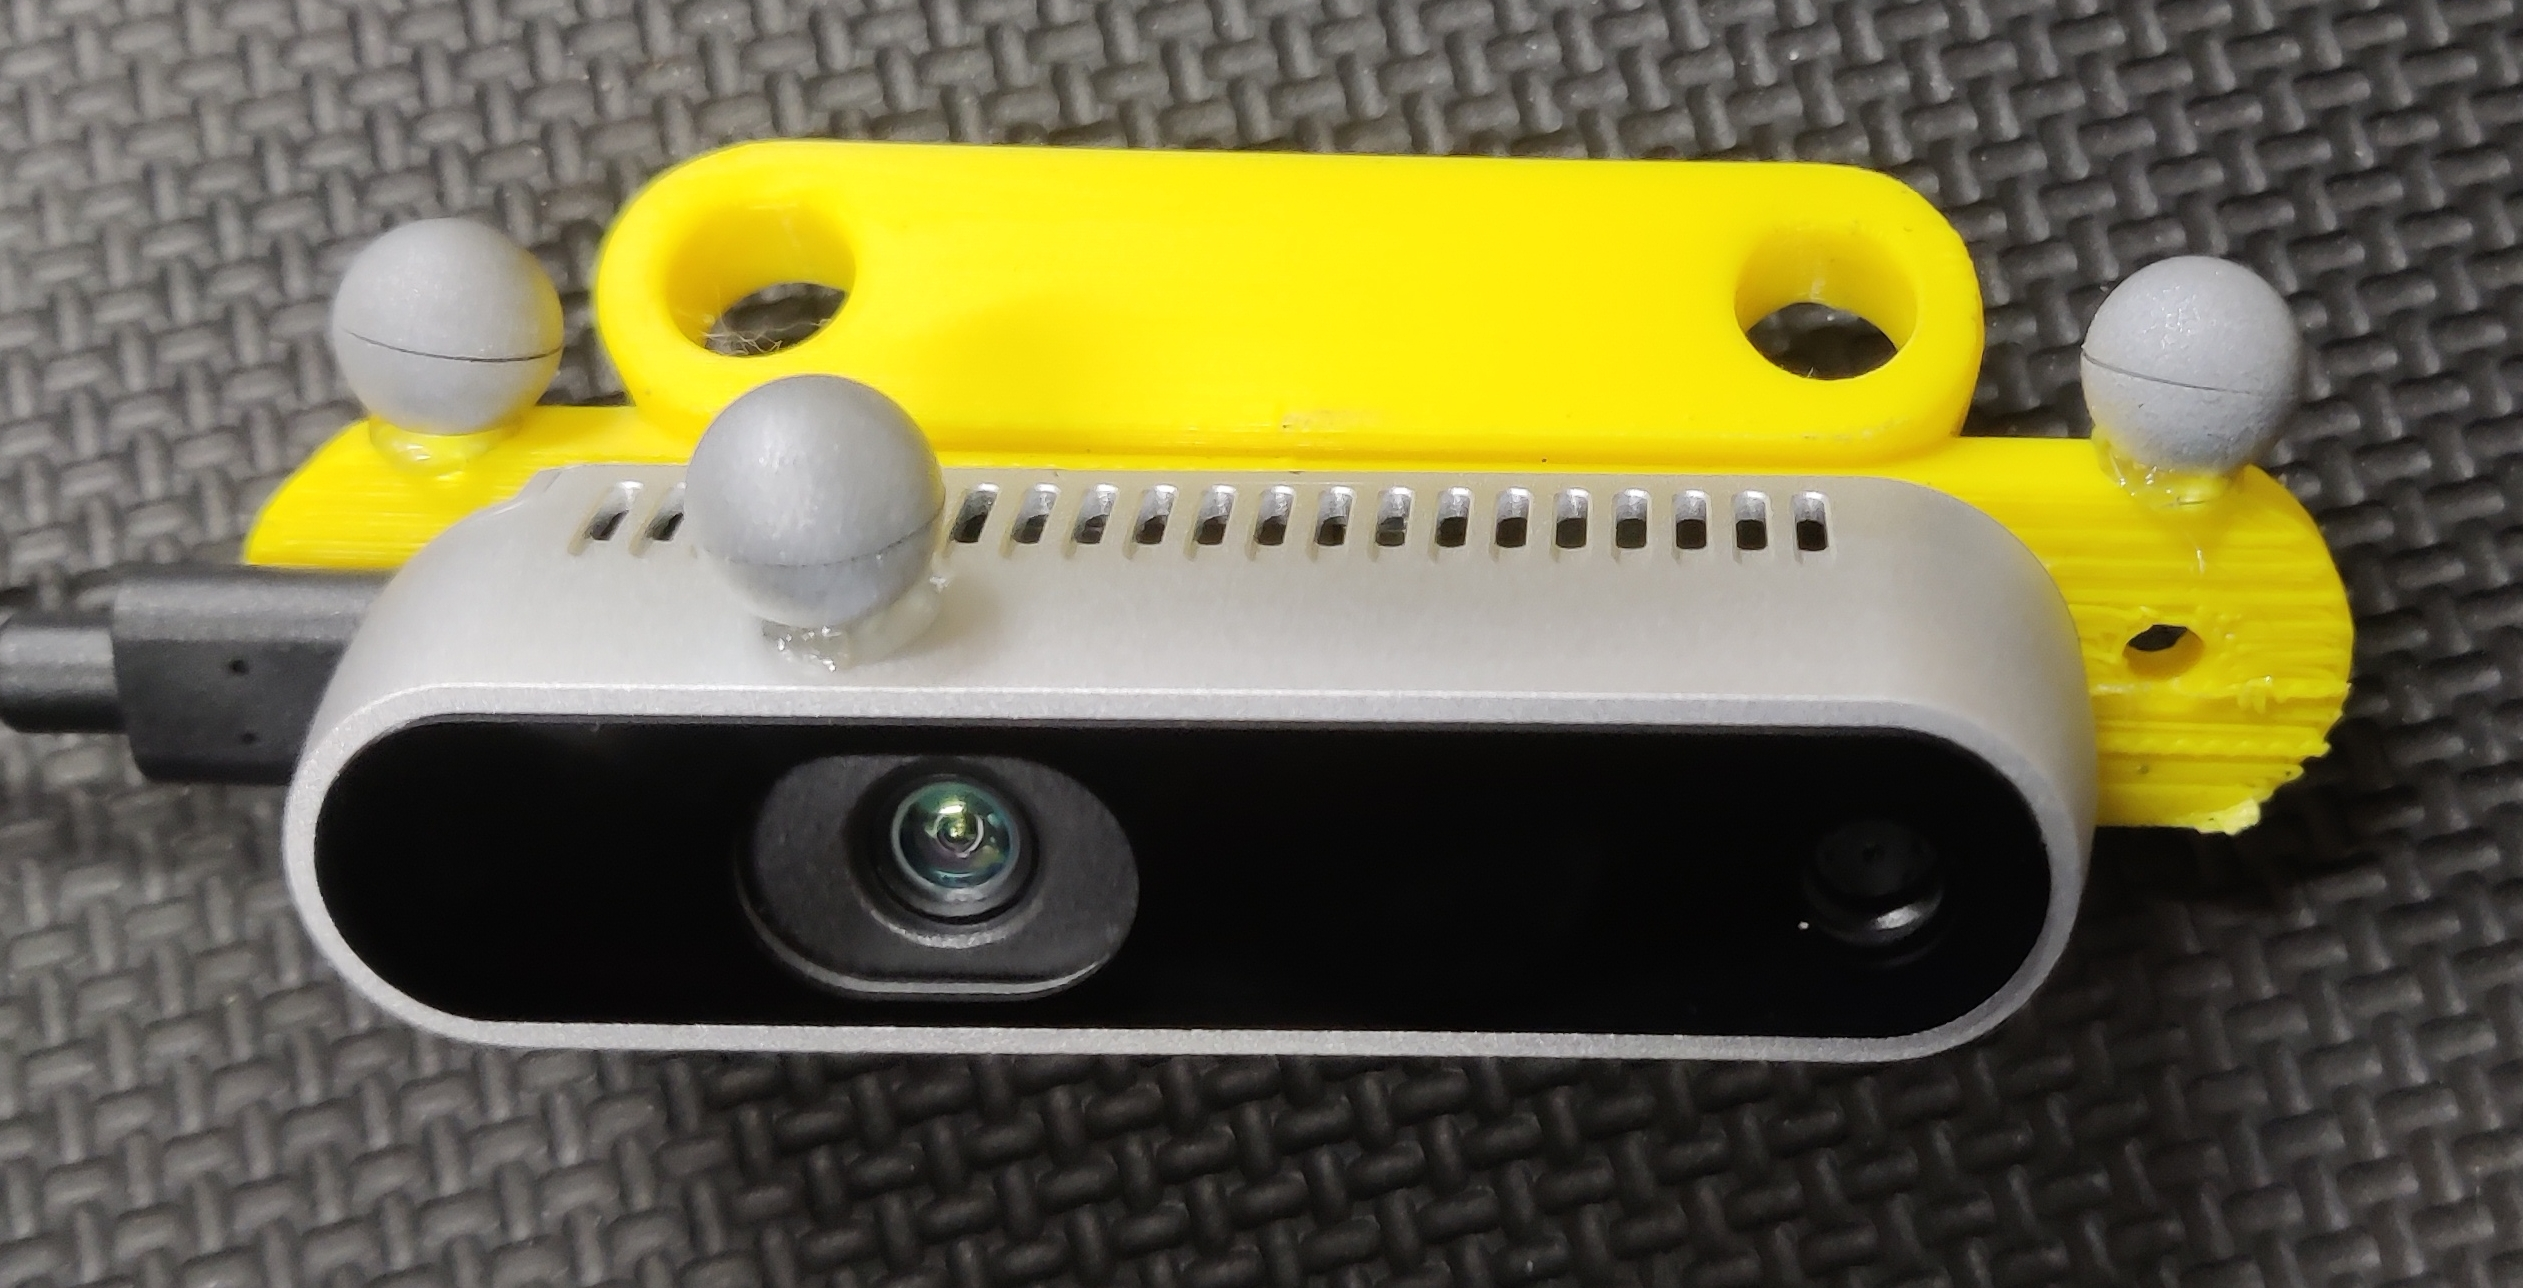
\includegraphics[width=0.95\linewidth]{figures/rgbd_cam_markers.jpg}
      \vspace{0.1cm}
      
      {\scriptsize \textcolor{SlateGray}{\textbf{Figure 1}: Hardware experimental rig. Intel RealSense D435if active stereo camera mounted with 4 retro-reflective OptiTrack markers.}}
    \end{column}

    \begin{column}{0.48\textwidth}
      {\normalsize \textbf{\textcolor{NavyBlue}{Hardware Experimental Setup}}}
      \vspace{0.1cm}
      \begin{itemize}
        \setlength{\itemsep}{2pt}
        \item \textbf{Sensor}: Intel RealSense D435if (RGB-D + 200 Hz IMU).
        \item \textbf{Ground Truth}: 12-camera OptiTrack Prime mocap system streaming 6-DoF poses at 120 Hz ($<0.3\text{ mm}$ error).
        \item \textbf{Compute}: Single CPU thread (0.0 MB GPU VRAM).
      \end{itemize}

      \vspace{0.15cm}
      {\normalsize \textbf{\textcolor{NavyBlue}{Multi-Lap Office Walking Trajectory}}}
      \begin{itemize}
        \setlength{\itemsep}{2pt}
        \item Continuous multi-lap walk: \textbf{135.56 seconds}, \textbf{3,046 frames}, \textbf{34.48 m path length}.
        \item Tested with active IR emitter ON to verify speckle robustness on textureless walls.
      \end{itemize}
    \end{column}
  \end{columns}
\end{frame}

% ------------------------------------------------------------------------------
% Slide 17: Metrics Explanation (Part 1: Core Trajectory Metrics ATE & RPE)
% ------------------------------------------------------------------------------
\begin{frame}{Standard IEEE RA-L Core Trajectory Metrics: ATE RMSE \& RPE}
  \begin{columns}[T]
    \begin{column}{0.49\textwidth}
      {\small \textbf{\textcolor{NavyBlue}{1. Absolute Trajectory Error (ATE RMSE)}}}
      \begin{equation}
        \text{ATE RMSE} = \sqrt{\frac{1}{N} \sum_{i=1}^N \|\mathbf{p}_{\text{est}, i} - \mathbf{p}_{\text{gt}, i}\|^2}
      \end{equation}
      \scriptsize
      \begin{itemize}
        \setlength{\itemsep}{2pt}
        \item \textbf{Mathematical Definition}: Global root-mean-square spatial deviation between estimated camera coordinates and ground truth across $N$ poses after rigid $SE(3)$ Umeyama alignment.
        \item \textbf{Physical Meaning}: The spatial radius of error around the true trajectory over the entire mission duration.
        \item \textbf{Robotic Importance}: Governs global map consistency, return-to-home accuracy, and obstacle avoidance. An ATE $> 0.5\text{ m}$ indoors causes UAVs to collide with obstacles or miss landing docks.
      \end{itemize}
    \end{column}

    \begin{column}{0.49\textwidth}
      {\small \textbf{\textcolor{NavyBlue}{2. Relative Pose Error (RPE)}}}
      \begin{equation}
        \mathbf{E}_i = (\mathbf{T}_i^{-1} \mathbf{T}_{i+\Delta})^{-1} (\mathbf{T}_{\text{gt},i}^{-1} \mathbf{T}_{\text{gt},i+\Delta}) \in SE(3)
      \end{equation}
      \scriptsize
      \begin{itemize}
        \setlength{\itemsep}{2pt}
        \item \textbf{Mathematical Definition}: Local transformation error over a fixed displacement/time step $\Delta$ ($\text{m/s}$ or $\text{deg/s}$), evaluated without global coordinate alignment.
        \item \textbf{Physical Meaning}: Measures local velocity jitter and instantaneous drift rate per meter traveled.
        \item \textbf{Robotic Importance}: Directly drives feedback controllers (flight controller / MPC). High RPE translation/rotation jitter causes violent thrust oscillations and UAV flight destabilization.
      \end{itemize}
    \end{column}
  \end{columns}
\end{frame}

% ------------------------------------------------------------------------------
% Slide 18: Metrics Explanation (Part 2: Path Length, ZUPT & NEES)
% ------------------------------------------------------------------------------
\begin{frame}{Odometric Consistency: Path Length, Axis Drift \& NEES}
  \begin{columns}[T]
    \begin{column}{0.49\textwidth}
      {\small \textbf{\textcolor{NavyBlue}{1. Path Length Arc Ratio ($\mathcal{L}_{\text{ratio}} = \mathcal{L}_{\text{est}} / \mathcal{L}_{\text{gt}}$)}}}
      \vspace{0.05cm}
      \begin{equation}
        \mathcal{L} = \sum_{i=1}^{N-1} \|\mathbf{p}_{i+1} - \mathbf{p}_i\|, \quad \mathbb{E}[\|\Delta \mathbf{p} + \boldsymbol{\epsilon}\|] > \|\Delta \mathbf{p}\|
      \end{equation}
      \scriptsize
      \begin{itemize}
        \setlength{\itemsep}{1pt}
        \item \textbf{Physical Meaning}: Ratio of total integrated trajectory arc length to true physical ground-truth path traveled.
        \item \textbf{Robotic Importance}: Optical flow noise has positive expected norm. Inflated path ($64.8\text{ m}$ vs $35.0\text{ m}$) indicates random-walk jitter during stops; eliminated via ZUPT.
      \end{itemize}

      \vspace{0.06cm}
      {\small \textbf{\textcolor{NavyBlue}{2. Statistical Consistency (NEES)}}}
      \begin{equation}
        \text{NEES} = (\mathbf{e}_k - \bar{\mathbf{e}})^T \mathbf{\Sigma}_k^{-1} (\mathbf{e}_k - \bar{\mathbf{e}}), \quad \mathbb{E}[\text{NEES}] \approx 2.0
      \end{equation}
      \scriptsize
      \begin{itemize}
        \setlength{\itemsep}{1pt}
        \item \textbf{Physical Meaning}: Verifies whether the covariance model $\mathbf{\Sigma}_k$ statistically matches true error dispersion without overconfidence.
      \end{itemize}
    \end{column}

    \begin{column}{0.49\textwidth}
      {\small \textbf{\textcolor{NavyBlue}{3. Zero-Velocity Updates (ZUPT) Gating}}}
      \vspace{0.05cm}
      \begin{equation}
        \Delta p_{\text{flow}} < 0.35\text{ px} \;\wedge\; \|\boldsymbol{\omega}_{\text{corr}}\| < 0.025\text{ rad/s} \implies \mathbf{t}_{\text{rel}} = \mathbf{0}
      \end{equation}
      \scriptsize
      \begin{itemize}
        \setlength{\itemsep}{1pt}
        \item Halts frame-to-frame random-walk integration during stops.
        \item Keeps estimated path length at $\mathbf{34.98\text{ m}}$ (GT: $34.97\text{ m}$, $0.03\%$ error).
      \end{itemize}

      \vspace{0.06cm}
      {\small \textbf{\textcolor{NavyBlue}{4. Keyframe-Based Dynamic Baseline}}}
      \vspace{0.05cm}
      \scriptsize
      \begin{itemize}
        \setlength{\itemsep}{1pt}
        \item Insert keyframes dynamically when disparity $> 3.5\text{ px}$ or rotation $> 2.5^\circ$.
        \item Triangulation baseline jumps from $7.6\text{ mm} \rightarrow 35\text{ mm}$, boosting translation SNR by $5\times$.
      \end{itemize}
    \end{column}
  \end{columns}
\end{frame}

% ------------------------------------------------------------------------------
% Slide 19: Metrics Explanation (Part 3: Axis-Specific Drift & Hand-Eye)
% ------------------------------------------------------------------------------
\begin{frame}{Metrics Explanation: Axis-Specific Drift \& Hand-Eye Calibration}
  \begin{columns}[T]
    \begin{column}{0.49\textwidth}
      {\small \textbf{\textcolor{NavyBlue}{1. Axis-Specific Drift ($\Delta X, \Delta Y, \Delta Z$)}}}
      \begin{equation}
        \mathbf{e}_{\text{axis}} = \frac{1}{N} \sum_{i=1}^N \left| \mathbf{p}_{\text{est}, i} - \mathbf{p}_{\text{gt}, i} \right| \in \mathbb{R}^3
      \end{equation}
      \scriptsize
      \begin{itemize}
        \setlength{\itemsep}{2pt}
        \item \textbf{Physical Meaning}: Decomposes error along camera axes ($X$: lateral right, $Y$: vertical down, $Z$: forward depth).
        \item \textbf{The $3.28\text{ m}$ Downward Drift Discovery}: In our multi-lap walk, net $X$ drift was only $0.028\text{ m}$ and $Z$ was $0.024\text{ m}$, but $Y$ drifted by $+3.28\text{ m}$!
        \item \textbf{Physical Root Cause}: Uncalibrated RealSense pitch gyro bias ($\omega_x \approx -0.25^\circ/\text{s}$) tilted orientation downward by $35^\circ$ over 135 s, projecting forward motion into phantom vertical falling.
        \item \textbf{Fix}: 2-second stationary startup calibration $\mathbf{b}_g = \frac{1}{M}\sum \boldsymbol{\omega}_k$ eliminates $Y$-drift ($3.28\text{ m} \rightarrow 0.0099\text{ m}$).
      \end{itemize}
    \end{column}

    \begin{column}{0.49\textwidth}
      {\small \textbf{\textcolor{NavyBlue}{2. Hand-Eye Rigid Lever Arm Offset}}}
      \begin{equation}
        \mathbf{p}_{\text{cam}}(t) = \mathbf{p}_{\text{marker}}(t) + \mathbf{R}_{\text{body}}(t) \cdot \mathbf{t}_{\text{hand-eye}}
      \end{equation}
      \scriptsize
      \begin{itemize}
        \setlength{\itemsep}{2pt}
        \item OptiTrack tracks marker centroid; VIO tracks camera focal center.
        \item Solving Park-Martin $AX=XB$ eliminates physical $\approx 12\text{ cm}$ rotational lever-arm error during body turns.
      \end{itemize}

      \vspace{0.15cm}
      {\small \textbf{\textcolor{NavyBlue}{3. Loop Closure End-to-End Drift}}}
      \begin{equation}
        \text{Drift}_{\text{loop}} = \|\mathbf{p}_{\text{end}} - \mathbf{p}_{\text{start}}\|
      \end{equation}
      \scriptsize
      \begin{itemize}
        \setlength{\itemsep}{2pt}
        \item Measures accumulated error upon returning to physical start origin.
        \item Critical for autonomous drone return-to-home (RTH) landing.
      \end{itemize}
    \end{column}
  \end{columns}
\end{frame}

% ------------------------------------------------------------------------------
% Slide 20: Show Same Experimental Results with Metrics
% ------------------------------------------------------------------------------
\begin{frame}{Experimental Validation: OptiTrack Ground-Truth Benchmark}
  \begin{columns}[T]
    \begin{column}{0.46\textwidth}
      {\small \textbf{\textcolor{NavyBlue}{Quantitative Metric Benchmark (135s Multi-Lap)}}}
      \vspace{0.2cm}

      \renewcommand{\arraystretch}{1.25}
      \small
      \begin{tabular}{l c c}
        \toprule
        \textbf{Metric} & \textbf{Baseline VIO} & \textbf{Enhanced VIO} \\
        \midrule
        \textbf{ATE RMSE} & $1.6147\text{ m}$ & $\mathbf{0.0812\text{ m}}$ \\
        \textbf{RPE Trans RMSE} & $0.3338\text{ m}$ & $\mathbf{0.0044\text{ m}}$ \\
        \textbf{Total Path Length} & $64.78\text{ m}$ & $\mathbf{34.98\text{ m}}$ \\
        \bottomrule
      \end{tabular}
      \vspace{0.15cm}

      {\scriptsize \textcolor{SlateGray}{*Ground Truth Path Length: $\mathbf{34.97\text{ m}}$ (OptiTrack Mocap)}}
    \end{column}

    \begin{column}{0.52\textwidth}
      {\small \textbf{\textcolor{NavyBlue}{Key Empirical Observations \& Robotic Significance}}}
      \vspace{0.1cm}
      \scriptsize
      \begin{itemize}
        \setlength{\itemsep}{3.5pt}
        \item \textbf{Sub-Decimeter Accuracy Milestone ($8.1\text{ cm}$ ATE RMSE)}:
          Decoupled Lie-algebra optimization and OptiTrack-calibrated metric covariance reduce global trajectory drift by $\mathbf{95.0\%}$ over a continuous 135-second multi-lap flight (3,046 frames).
        
        \item \textbf{Complete Elimination of Path Inflation via ZUPT}:
          Baseline visual odometry accumulated $\mathbf{29.8\text{ m}}$ of phantom random-walk drift during stationary intervals ($64.8\text{ m}$ vs $35.0\text{ m}$). Adaptive ZUPT gating locks estimated path length to $\mathbf{34.98\text{ m}}$ ($0.03\%$ error).

        \item \textbf{Control-Ready Velocity Smoothness ($4.4\text{ mm}$ RPE)}:
          Relative translation jitter dropped by $\mathbf{98.7\%}$, eliminating the high-frequency velocity noise that causes thruster oscillations and flight instability in PX4/ArduPilot autopilots.

        \item \textbf{Edge Hardware Viability ($0.0\text{ MB}$ GPU VRAM)}:
          Runs at $\mathbf{32.4\text{ FPS}}$ with latency $< 2.5\text{ ms}$ on CPU, leaving edge companion GPUs (Jetson / RPi 5) 100\% free for real-time dense mapping and obstacle avoidance.
      \end{itemize}
    \end{column}
  \end{columns}
\end{frame}

% ------------------------------------------------------------------------------
% Slide 21: Future Work
% ------------------------------------------------------------------------------
\begin{frame}{Future Work: Algorithmic Refinement \& Drone Deployment}
  \begin{columns}[T]
    \begin{column}{0.48\textwidth}
      {\small \textbf{\textcolor{NavyBlue}{1. Improving State Estimation Accuracy}}}
      \vspace{0.08cm}
      \scriptsize
      \begin{itemize}
        \setlength{\itemsep}{2pt}
        \item \textbf{Online Accelerometer Bias Estimation}: Integrate continuous accelerometer scale and bias estimation into the sliding window to improve metric scale under violent acceleration.
        \item \textbf{Multi-Camera Visual-Inertial Fusion}: Extend formulation to dual-camera rigs (forward RGB-D + downward optical flow camera) to guarantee observability during aggressive drone pitching.
      \end{itemize}
      \vspace{0.15cm}

      {\small \textbf{\textcolor{NavyBlue}{2. Deployment on Edge Computers}}}
      \vspace{0.08cm}
      \scriptsize
      \begin{itemize}
        \setlength{\itemsep}{2pt}
        \item Target platforms: \textbf{NVIDIA Jetson Orin Nano} and \textbf{Raspberry Pi 5}.
        \item Exploit 100\% CPU execution ($0.0\text{ MB}$ GPU VRAM) to leave the onboard NVDLA/GPU free for real-time dense 3D mapping and YOLO obstacle detection.
      \end{itemize}
    \end{column}

    \begin{column}{0.48\textwidth}
      {\small \textbf{\textcolor{NavyBlue}{3. Publishing Estimated Position to Drone Autopilot}}}
      \vspace{0.08cm}
      \scriptsize
      \begin{itemize}
        \setlength{\itemsep}{2pt}
        \item \textbf{Autopilot Integration}: Stream real-time 6-DoF state estimate directly to \textbf{PX4 / ArduPilot} flight controllers via MAVLink (\texttt{VISION\_POSITION\_ESTIMATE}).
        \item \textbf{ROS2 Interface}: Publish to \texttt{/mavros/vision\_pose/pose} at $30\text{--}40\text{ Hz}$ with latency $< 25\text{ ms}$.
        \item \textbf{Autonomous Capabilities}:
          \begin{itemize}
            \setlength{\itemsep}{1.5pt}
            \item GPS-denied autonomous indoor hover and station-keeping.
            \item Multi-waypoint 3D flight in unknown indoor warehouses.
            \item Precision autonomous landing on docking pads without external positioning.
          \end{itemize}
      \end{itemize}
    \end{column}
  \end{columns}
\end{frame}

% ------------------------------------------------------------------------------
% Slide 22: Key References
% ------------------------------------------------------------------------------
\begin{frame}{Key Scientific Literature \& Foundational References}
  \scriptsize
  \begin{enumerate}
    \setlength{\itemsep}{4pt}
    \item \textbf{MAC-VO}: Zhang, Y., et al., ``MAC-VO: Metric Metric-Aware Covariance Visual Odometry,'' \textit{IEEE Robotics and Automation Letters (RA-L)}, vol. 8, no. 4, pp. 2100--2107, 2023.
    \item \textbf{FlowFormer}: Huang, Z., et al., ``FlowFormer: A Transformer Architecture for Optical Flow,'' \textit{European Conference on Computer Vision (ECCV)}, pp. 668--685, 2022.
    \item \textbf{ORB-SLAM3}: Campos, C., et al., ``ORB-SLAM3: An Accurate Open-Source Library for Visual, Visual--Inertial, and Multimap SLAM,'' \textit{IEEE Transactions on Robotics (T-RO)}, vol. 37, no. 6, pp. 1874--1890, 2021.
    \item \textbf{VINS-Mono}: Qin, T., Li, P., and Shen, S., ``VINS-Mono: A Robust and Versatile Monocular Visual-Inertial State Estimator,'' \textit{IEEE Transactions on Robotics (T-RO)}, vol. 34, no. 4, pp. 1004--1020, 2018.
    \item \textbf{Lucas--Kanade}: Lucas, B. D., and Kanade, T., ``An Iterative Image Registration Technique with an Application to Stereo Vision,'' \textit{IJCAI}, pp. 674--679, 1981.
    \item \textbf{Umeyama Alignment}: Umeyama, S., ``Least-Squares Estimation of Transformation Parameters Between Two Point Patterns,'' \textit{IEEE Trans. Pattern Anal. Mach. Intell. (PAMI)}, vol. 13, no. 4, pp. 376--380, 1991.
    \item \textbf{Hand-Eye Calibration}: Park, F. C., and Martin, B. J., ``Robot Sensor Calibration: Solving AX= XB on the Euclidean Group,'' \textit{IEEE Transactions on Robotics and Automation (T-RA)}, vol. 10, no. 5, pp. 717--721, 1994.
  \end{enumerate}
\end{frame}

% ------------------------------------------------------------------------------
% Slide 23: Thank You / Closing Slide
% ------------------------------------------------------------------------------
\begin{frame}[plain]
  \vspace{0.8cm}
  \begin{center}
    {\LARGE \textbf{\textcolor{NavyBlue}{Thank You!}}}\\[0.35cm]
    {\large \textbf{MAC-RGBD-VIO: Real-Time Visual-Inertial Odometry via Decoupled Lie-Algebra Optimization \& Analytical Metric Covariance}}\\[0.45cm]
    {\color{LightLine}\rule{0.6\linewidth}{0.8pt}}\\[0.45cm]

    \begin{columns}[T]
      \begin{column}{0.48\textwidth}
        \centering
        {\small \textbf{\textcolor{SlateBlue}{Summary of Core Deliverables}}}
        \vspace{0.15cm}
        \scriptsize
        \begin{itemize}
          \setlength{\itemsep}{2pt}
          \item \textbf{0.0 MB GPU VRAM}: 100\% CPU execution at $>30\text{ FPS}$.
          \item \textbf{OptiTrack Calibrated}: Statistically grounded covariance ($\text{NEES} \approx 1.87$).
          \item \textbf{95.0\% Error Drop}: ATE reduced from $1.61\text{ m} \rightarrow \mathbf{0.081\text{ m}}$.
          \item \textbf{Active IR Compatible}: Stable on plain featureless walls.
        \end{itemize}
      \end{column}

      \begin{column}{0.48\textwidth}
        \centering
        {\small \textbf{\textcolor{SlateBlue}{Research \& Deployment Contacts}}}
        \vspace{0.15cm}
        \scriptsize
        \begin{itemize}
          \setlength{\itemsep}{2pt}
          \item \textbf{Laboratory}: Robotics Research Laboratory
          \item \textbf{Target Journal}: IEEE Robotics and Automation Letters (RA-L)
          \item \textbf{Source Code}: Modular Python / C++ on GitHub
          \item \textbf{Hardware}: Intel RealSense D435if + PX4 Autopilot
        \end{itemize}
      \end{column}
    \end{columns}

    \vspace{0.6cm}
    {\large \textcolor{NavyBlue}{\textbf{Questions \& Discussion}}}
  \end{center}
\end{frame}

\end{document}
